\chapter{常用的图像增强方法}\label{chap:otherAlgorithms}本章首先介绍直方图均衡增强算法和Retinex增强算法的基本原理和发展历程,阐述他们在航空图像增强中的应用。	

		\section{直方图均衡}
			\subsection{直方图均衡增强算法理论}直方图均衡通常会增加许多图像的全局对比度,特别是当图像的可用数据由近似对比值表示时。通过这种调整,直方图上的强度可以更好地分布,使局部对比度较低的区域获得较高的对比度。直方图均衡通过有效地分散最频繁的强度值来实现这一点。该方法在背景和前景都很亮或两者都暗的图像中很有用。例如,该方法可以更好地观察X射线图像中的骨骼结构,并可以更好地了解曝光过度或曝光不足的照片的细节。该方法的一个关键优点是它是一种相当直接的技术和可逆运算符。所以理论上,如果直方图均衡函数是已知的,那么原始直方图可以被恢复。该方法的一个缺点它可能增加背景噪声的对比度,同时减少可用信息。

直方图均衡算法的改进是使用多个直方图(称为子图)来强调局部对比度,而不是整体对比度。直方图均衡改进算法包括自适应直方图均衡化,对比限制自适应直方图均衡化,多峰直方图均衡化和多用途$\beta$优化生物统计图均衡化。这些方法的目标,是通过改进HE算法来改善对比度而不产生亮度均值偏移和细节损失伪影。直方图均衡化的信号变换也在生物神经网络有所应用,作为输入统计量的函数使神经元的输出发放速率最大化。
直方图均衡是一般的直方图重新映射方法的一个特例。这些方法试图调整图像以使其更容易分析或改善视觉质量,例如Retinex。
			\subsection{直方图均衡增强算法实现}直方图描述了一幅图像的绘图统计信息,是一个关于灰度的函数,如令$x$表示灰度值,则离散函数$f(x)$表示当$x$为特定灰度值时,一幅图像上灰度值为$x$的像素的数量。

直方图均衡属于图像增强技术中的空域方法,即直接对像素值施加以相应的操作以获得增强效果。直方均衡是一种利用图像的直方图像来调整图像对比度的一项技术,该技术基于将原场景图像的直方图经重新映射后得到一个接近于均匀分布的概率密度函数的新的直方图的思想,是一种简单有效的对比度拉伸技术\cite{?}。	

直方图均衡的目的是使原始图像原有的灰度分布即直方图,重新在一定的范围内“均匀”分布。而对于原始图像直方图具有的谷值和峰值,直方图均衡处理后仍具有原来的形状,并且变得平滑。以下将阐述直方图均衡的数学表达。

考虑连续的灰度值,用r表示原始出翔的灰度。假设r的取值区间是$[0,L-1]$,灰度值变换公式为
\begin{equation}s=T(r),0 \leq r\leq L-1 \end{equation}
%\begin{eqnarray*}
%x^n+y^n &=& z^n \\
%x+y &=& z
%\end{eqnarray*}
%其中两个&号之间的是公式间对齐的位置,用\\隔开各行公式。上面输出的公式是没有编号的,如果需要自动编号,可以将eqnarray*改为eqnarray 。 

灰度变换公式满足以下条件
			\begin{itemize}
				\item \emph{$T(r)$在区间$0\leq r\leq L-1$上为单调递增函数。}
				\item \emph{当$0\leq r\leq L-1$时,$0\leq T(r) \leq L-1$。}
			\end{itemize}

原始图像的灰度值可视为$[0,L-1]$内的随机变量。用概率密度函数(probability density function,PDF)来描述这些随机变量。有如下公式:
\begin{equation}p_s(s)=p_r(r)|\frac{dr}{ds}|\end{equation}	
其中$p_r(r)$表示随机变量$r$的概率密度函数,$p_s(s)$表示随机变量$s$的概率密度函数。并有如下公式:
\begin{equation}     s=T(r)=(L-1)\int_0^r p_r(v)\,dv    \end{equation}	
\begin{equation}     \frac{ds}{dr}=\frac{dT(r)}{dr}=(L-1)\frac{d}{dr}\left[\int_0^r p_r(v)\,dv 	\right]=(L-1)P_r(r)     \end{equation}
\begin{equation}     p_s(s)=p_r(r) \left| \frac{dr}{ds}\right| =p_r(r) \left| \frac{1}{(L-1)p_r(r)} \right| = \frac{1}{L-1},0 \leq s \leq L-1    \end{equation}
其中,v是积分假变量。公式的右边是随机变量$r$的累计分布函数(cumulative distribution function, CDF)。由公式$(2.5)$得知得到的$p_s(s)$始终是均匀的,与$P_r(r)$无关。简单的来说就是使原始图像的灰度直方图的累计分布函数均匀分布使得原始图像的对比度变高。以下是一个直方图均衡的例子:

\begin{figure}[!htbp]
    \centering
    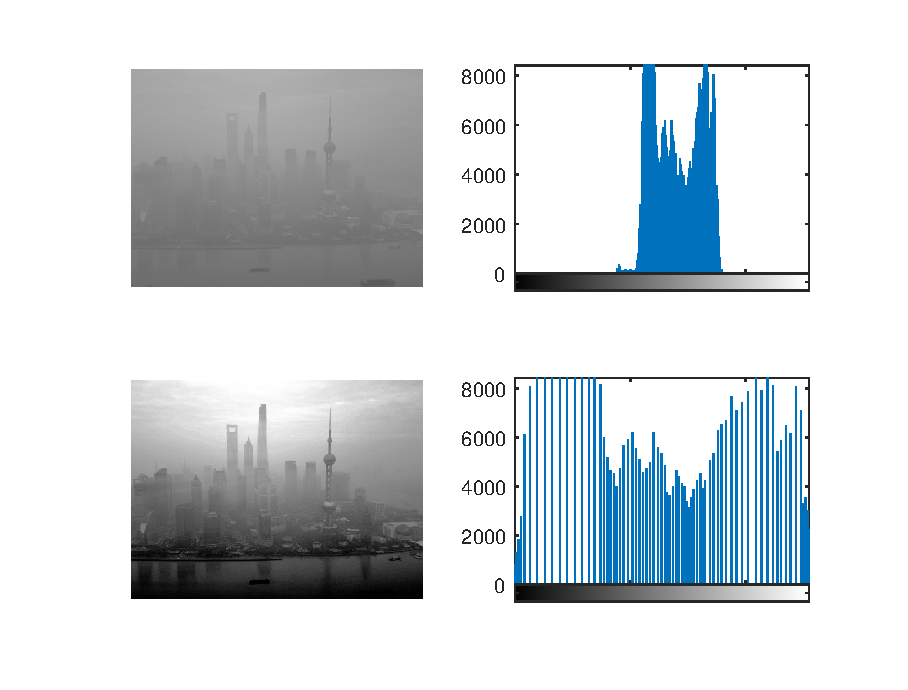
\includegraphics[width=0.40\textwidth]{histogramExample}
    \bicaption{Q判据等值面图,同时测试一下一个很长的标题,比如这真的是一个很长很长很长很长很长很长很长很长的标题。}{Isocontour of Q criteria, at the same time, this is to test a long title, for instance, this is a really very long very long very long very long very long title.}
    \label{fig:tc_q_criteria}
\end{figure}

从上图可以看出原本对比度很低,模糊不清的原始图像经过直方图均衡后变得更为清晰,视觉效果好。其中,均衡化后图像的灰度直方图形状与原图的灰度直方图相似,只不过被“拉伸"了。直方图均衡有助于图像的增强,但是也有过增强和细节变得更加模糊的缺点。

虽然直方图均衡化后的效果比原始图像好,但是所得的图像在一些轮廓和细节方面处理是不如其他常用的增强算法的,会产生轮廓的模糊等现象。
		\section{Retinex增强算法}	Retinex(Retina-Cortex)理论是在1977年由Edwin Land提出的关于图像增强的理论,器阐述了人通过亮度感知捕捉色度图像在不同亮暗情况下辨认物体的能力。是研究人员模仿人类视觉系统而发展而成的算法,从单尺度Retinex(Single Scale Retinex,ssr)算法改进成多尺度加权平均的Retinex算法(Multi Scale Retinex,msr),再发展成彩色恢复多尺度Retinex算法。由于人眼对亮度、饱和度、对比度拥有相当的分辨能力,基于肉眼视觉感受的航空图像增强有助于观察者分析并且观察航空图像,并从中获取预期的信息和得到预期的视觉效果。Retinex理论包含两个方面的内容:$(1)$物体的色彩具有一致性,不受光的非均匀性的影响。$(2)$物体的颜色不是取决于反射光的强度的绝对值,而是取决于物体对各种波长的发射能力决定的。

Retinex理论通常广泛在可见光图像增强领域有所应用,而航空图像正好可以运用Retinex理论进行分析和处理。一下将介绍有关颜色视觉理论和肉眼视觉的特性的相关知识。
			\subsection{颜色视觉理论和人眼视觉特性}
				\subsubsection{人眼视觉特性}眼睛是一个接受神经系统以及大脑调节和控制的一个复杂光学系统。在长期的生物进化过程中,人类形成了独有的视觉特性,以便适应自然环境以及加强对物体的感知。眼睛的视觉特性有以下几个特点:
				\begin{itemize}
					\item \emph{波长位于$400~800nm$的电磁波是人的眼睛可以看见的电磁波,在这范围内的电磁波也可被称为白光。七色光就是白光通过三棱镜折射而成的。}
					\item \emph{人的眼睛对不同波段的可见光的敏感程度是不一样的,其中对于黄绿光所在波段的电磁波的敏感度较高,而对红蓝光所在波段的电磁波的敏感度较低。}
					\item \emph{人的眼睛对亮度和光强的响应不是线性的。只有光强到一定的阈值时,人的眼睛才能感知光强的变化,并且在黑暗环境下人的眼睛对于光强和亮度的变化比明亮环境下的更敏感。}
					\item \emph{人的眼睛对与细节的分辨能力是有限的。比如,当移动的目标速度变快时,肉眼分辨率下降。}
					\item \emph{对目标亮度和色彩的感知与背景相关。}
				\end{itemize}

通过研究人的眼睛的视觉特性有助于建立相对应的视觉模型,如黑白模型,彩色视觉模式等视觉模型。这些视觉模型的建立应用于图像增强领域以帮助提高人对图像的视觉能力,增强分辨力。
				\subsubsection{颜色视觉理论}彩色视觉色觉是有机体或机器基于其反射、发射或传播的光的波长(或频率)区分物体的能力。 颜色可以通过各种方式进行测量和量化; 事实上,一个人对色彩的感知是一个主观过程,大脑响应当入射光与眼睛中几种类型的视锥细胞反应时产生的刺激。 实质上,不同的人以不同的方式看到相同的照明物体或光源。

色彩视觉的两个互补理论是三色理论和对手过程理论。 Thomas Young和Hermann von Helmholtz在19世纪提出的三色理论或Young-Helmholtz理论指出,视网膜的三种类型的视锥优先对蓝色,绿色和红色敏感。 Ewald Hering在1872年提出了对手过程理论。 它指出,视觉系统以对立的方式解释颜色:红色与绿色,蓝色与黄色,黑色与白色。 这两种理论现在都被认为是有效的,描述了视觉生理学的不同阶段。
光的波长范围以不同程度刺激这些受体类型中的其中一种。例如,黄绿色的光线同样强烈地刺激L和M锥体,但仅仅弱地刺激S锥体。另一方面,红光刺激L锥体比M锥体多得多,而S锥体几乎不刺激;蓝绿光与L锥相比更能刺激M锥,S锥更强烈,也是棒状细胞的高峰兴奋剂;蓝光比红光或绿光更强烈地刺激S锥,但L和M锥更弱。大脑结合了来自每种类型受体的信息,从而产生对不同波长光的不同感知。

存在于L和M视锥中的视蛋白(光敏色素)在X染色体上编码;这些缺陷编码导致两种最常见的色盲形式。编码L型视蛋白中的视蛋白的OPN1LW基因具有高度多态性。很小比例的女性可能有一种额外类型的彩色受体,因为它们在每个X染色体上具有用于L视蛋白基因的不同等位基因。 X染色体失活意味着虽然在每个视锥细胞中仅表达一种视蛋白,但这两种类型都是整体出现的,并且一些女性可能因此显示一定程度的四色视觉[10]。在编码以M个锥体表达的视蛋白的OPN1MW中的变异似乎很少,观察到的变体对光谱灵敏度没有影响。

通过初始颜色对手机制,颜色处理在视觉系统中(甚至在视网膜内)以非常早的水平开始。因此,亥姆霍兹的三色理论和霍林的反对过程理论都是正确的,但三色性在受体水平上出现,并且对立过程出现在视网膜神经节细胞及其以外的水平。在Hering的理论中,对手机制指的是红绿,蓝黄和明暗的相反颜色效应。然而,在视觉系统中,反对的是不同受体类型的活性。一些侏儒视网膜神经节细胞反对L和M锥体活动,其对应于松散的红绿对称性,但实际上沿着从蓝绿色到品红色的轴线延伸。小双分子视网膜神经节细胞反对从S锥体输入来自L和M锥体的输入。这通常被认为对应于蓝黄色的对数,但实际上沿着从黄绿色到紫色的颜色轴。

颜色恒常性是主观恒定性的一个例子,是人类色彩感知系统的一个特征,它确保在变化的照明条件下物体的感知颜色保持相对恒定。 例如,当主要照明为白色阳光时,以及在日落时主要照明为红色时,例如一个青苹果在中午看起来为绿色。 这有助于我们识别物体。

				\subsection{单尺度Retinex}单尺度Retinex算法是在色彩恒常性基础上,经过人眼模拟获得图像的信息的过程,图像模型转化为场景反射和光照分布两个过程。具体流程和算法图下所示:

一幅给定图像$s(x,y)$可以分解为两个不同的图像:反射图像$r(x,y)$和亮度图像$L$,原理图如下:

\begin{figure}[!htbp]
    \centering
    \includegraphics[width=0.40\textwidth]{retinexSSR}
    \bicaption{Q判据等值面图,同时测试一下一个很长的标题,比如这真的是一个很长很长很长很长很长很长很长很长的标题。}{Isocontour of Q criteria, at the same time, this is to test a long title, for instance, this is a really very long very long very long very long very long title.}
    \label{fig:tc_q_criteria}
\end{figure}

%			\begin{figure}[!ht]\centering
%				\includegraphics[totalheight=60mm]{./figures/retinexSSR.png}
%				\caption{SSR原理图\label{SSR}}
%			\end{figure}

如上图所示,入射光照射在反射物体上,通过反射物体的反射形成反射光进入人眼,得到人所见到的图像,用公式表达为:
\begin{equation}     S(x,y)=R(x,y)L(x,y)    \end{equation}	
其中,$L(x,y)$表示入射图像,他决定了图像中像素多能达到的动态范围,$R(x,y)$表示物体的反射性质图像,即图像的内在属性,$S(x,y)$表示人眼所能接收到的反射光图像。该理论的基本思想是在原始图像中,通过某种方法降低或去除入射图像的影响,从而尽可能保留物体本质的反射属性图像。其一般处理过程如下所示:


\begin{figure}[!htbp]
    \centering
    \includegraphics[totalheight=30mm,width=160mm]{retinexSSR}
    \bicaption{Q判据等值面图,同时测试一下一个很长的标题,比如这真的是一个很长很长很长很长很长很长很长很长的标题。}{Isocontour of Q criteria, at the same time, this is to test a long title, for instance, this is a really very long very long very long very long very long title.}
    \label{fig:tc_q_criteria}
\end{figure}
%			\begin{figure}[!ht]\centering
%				\includegraphics[totalheight=30mm,width=160mm]{./figures/retinexSSR1.png}
%				\caption{SSR原理图(这个图像要改)\label{SSR}}
%			\end{figure}

我们把照射图像假设为空间平滑图像,可得单尺度Retinex算法公式为:
\begin{equation}     r(x,y)=logR(x,y)=log \frac{S(x,y)}{L(x,y)}    \end{equation}
\begin{equation}     r(x,y)=logS(x,y)-log \left[ F(x,y)*S(x,y) \right]    \end{equation}	
\begin{equation}     F(x,y)=\lambda e^{\frac{-(x^2+y^2)}{c^2}}    \end{equation}	

其中,$r(x,y)$为输出图像,$*$为卷积符号,$F(x,y)$为中心环绕函数,$c$表示高斯环绕尺度,$\lambda$是一个尺度,中心环绕函数$F(x,y)$的取值要满足
\begin{equation}     \int\int F(x,y)\,dx \,dy=1    \end{equation}

可以从上面的式子中看出SSR算法中的卷积可以看作是对空间中照度图像的计算,它的物理意义可以表示为通过计算图像中像素点和周围区域在加权平均来估计图像中照度的变化,并将其去除,最后只保留图像中物体的反射属性,从而达到增强的目的。中心环绕函数$F(x,y)$采用低通函数,能够在算法中估计出照射图像所对应的原始图像的低频部分,留下对应的高频部分即边缘信息。所以SSR算法可以较好的增强图像中的边缘信息。以下将展示SSR算法的增强效果。

\begin{figure}[!htbp]
    \centering
    \includegraphics[totalheight=30mm,width=160mm]{SSR2}
    \bicaption{Q判据等值面图,同时测试一下一个很长的标题,比如这真的是一个很长很长很长很长很长很长很长很长的标题。}{Isocontour of Q criteria, at the same time, this is to test a long title, for instance, this is a really very long very long very long very long very long title.}
    \label{fig:tc_q_criteria}
\end{figure}

%			\begin{figure}[!ht]\centering
%				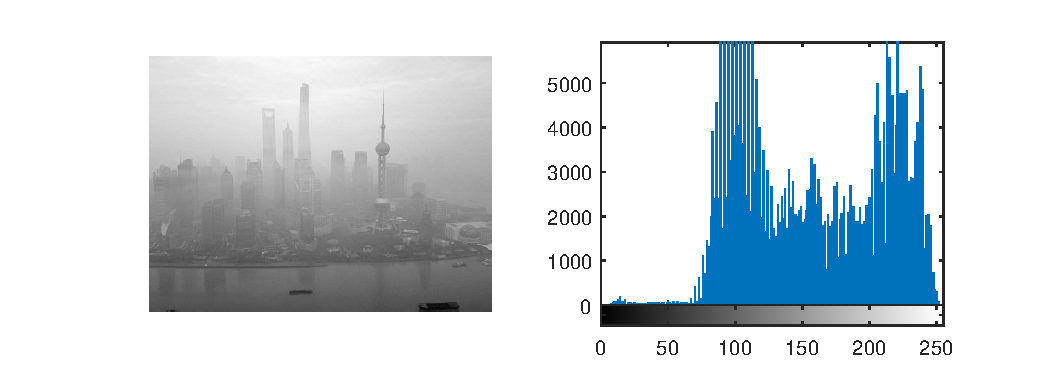
\includegraphics[totalheight=60mm]{./figures/ssr2.eps}
%				\caption{SSR增强算法\label{SSR}}
%			\end{figure}

从上图中可见,图2.4增强效果好,突出了图像细节,符合人眼感官。从图2.4的灰度直方图中可见,图中形状和图2.1中的灰度直方图相似,对比度加强,即同样被更加适当的“拉伸”了。